\chapter {Release 1 : Mise en place des fonctionnalités de base}

\section{Introduction} 
Dans ce chapitre, nous détaillerons le déroulement de la première Release. Nous débuterons par la présentation des backlogs des deux premiers sprints, accompagnée des diagrammes de classes correspondants. Ensuite, nous exposerons les diagrammes de cas d’utilisation illustrant les différentes fonctionnalités, ainsi que les diagrammes de séquence pour certaines tâches spécifiques liées à cette release. Pour conclure, nous proposerons un aperçu des interfaces des fonctionnalités développées durant cette phase.

\section{Sprint 1}
\subsection{Objectifs du sprint 1}
L'objectif de ce sprint est de mettre en place les fonctionnalités de base liées à l'authentification et à la gestion collaborative des groupes, afin d'assurer un accès sécurisé et une gestion collaborative des médicaments en famille ou en équipe soignante. Cela inclut la création de comptes utilisateurs, l'authentification sécurisée avec JWT, la réinitialisation de mot de passe et la vérification des comptes par code OTP. En complément, ce sprint introduit la gestion des groupes familiaux ou médicaux, permettant au gestionnaire de créer des groupes, d'ajouter des membres via QR code ou identifiant, de retirer des membres, et d'assigner des rôles (gestionnaire, responsable, membre) pour organiser la prise en charge médicale.

\subsection{Backlog sprint 1}
Le Sprint Backlog est un document vivant qui regroupe l'ensemble des éléments de travail sélectionnés pour être réalisés pendant un sprint. Il constitue l'engagement de l'équipe de développement à livrer une valeur incrémentale à la fin de l'itération.

\begin{table}[H]
\centering
\renewcommand{\arraystretch}{1.4}
\resizebox{\textwidth}{!}{%
\begin{tabular}{|
>{\centering\arraybackslash}m{1cm}|
>{\centering\arraybackslash}m{4cm}|
>{\centering\arraybackslash}m{1cm}|
m{6cm}|
>{\centering\arraybackslash}m{2cm}|
>{\centering\arraybackslash}m{2cm}|
>{\centering\arraybackslash}m{2cm}|}
\hline
\textbf{ID} & \textbf{Module} & \textbf{ID} & \textbf{User Story} & \textbf{Priorité} & \textbf{Complexité} & \textbf{Nb jours} \\
\hline

\multirow{3}{*}{1} & \multirow{3}{4cm}{Gestion des utilisateurs}
& 1.1 & En tant qu'utilisateur, je veux créer un compte & Haute & 3 & 2 \\
\cline{3-7}
& & 1.2 & En tant qu'utilisateur, je dois m'authentifier & Haute & 5 & 3 \\
\cline{3-7}
& & 1.3 & En tant qu'utilisateur, je veux réinitialiser mon mot de passe & Haute & 3 & 1 \\
\hline

\multirow{4}{*}{3} & \multirow{4}{4cm}{Gestion des groupes}
& 3.4 & En tant que gestionnaire, je veux ajouter un utilisateur à un groupe soit en scannant son QR code, soit en utilisant son identifiant & Haute & 5 & 4 \\
\cline{3-7}
& & 3.5 & En tant que gestionnaire, je veux retirer un utilisateur de mon groupe & Haute & 5 & 1 \\
\cline{3-7}
& & 3.7 & En tant que gestionnaire, je veux assigner un utilisateur en tant que responsable & Haute & 5 & 2 \\
\cline{3-7}
& & 3.8 & En tant que gestionnaire, je veux désassigner un utilisateur en tant que responsable & Haute & 5 & 1 \\
\hline

\end{tabular}%
}
\captionsetup{justification=centering}
\caption{Backlog sprint 1}
\label{tab:Backlog sprint 1}
\end{table}

Le tableau 3.1 représente le backlog de la première sprint.

\subsection{Etude Conceptuelle du sprint 1}
\subsubsection{Use Case du Sprint 1}
La figure 3.1 représnete la diagramme de cas d'utilisation du premier sprint "Authentification et gestion orgianisation et profil"

\begin{figure}[H]
    \centering
    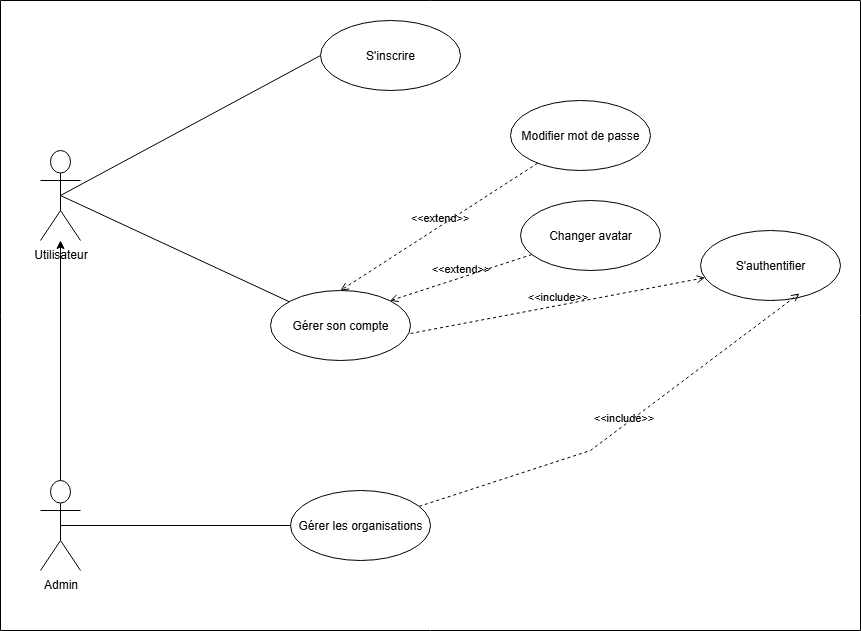
\includegraphics[width=1\linewidth]{img/useCaseSprint1.png}
    \caption{Diagramme de classes sprint 1}
    \label{fig:enter-label}
\end{figure}

\subsubsection{Digramme de classes Sprint 1}
Cette figure 3.2 représente le diagramme de classes qui répresente les classes et entités du système, leurs attributs, les méthodes,ainsi que les relations entre les entités.

\begin{figure}[H]
    \centering
    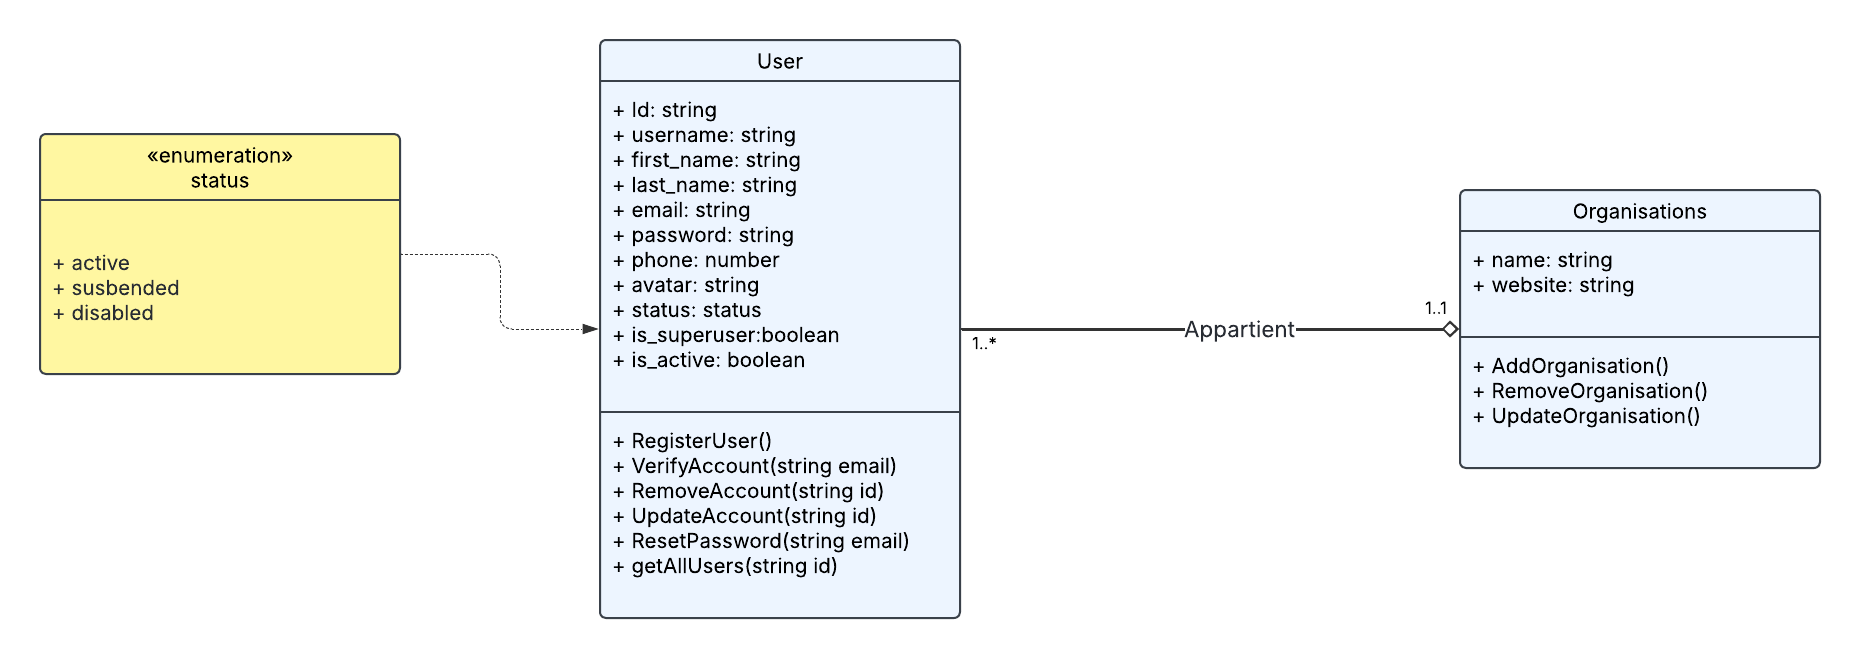
\includegraphics[width=1.15\linewidth]{img/Sprint 1 Classes FV.png}
    \caption{Diagramme de classes sprint 1}
    \label{fig:enter-label}
\end{figure}

\subsubsection{Descriptions textuelle des cas d’utilisation}
Cette partie vise à approfondir et détailler les cas d'utilisation, en mettant en évidence les processus essentiels ainsi que les interactions clés entre les utilisateurs et le système.

\paragraph{Cas d’utilisation "S’inscrire"}

\begin{itemize} [label=\textbullet]
    \item \textbf{Description textuelle du cas d’utilisation S’inscrire}
\end{itemize}

Ce tableau 3.2 représente la description textuelle du cas d'utilisation "S'inscrire"

\begin{longtable}{|>{\raggedright\arraybackslash}p{4cm}|>{\raggedright\arraybackslash}p{11cm}|}
\hline
\textbf{Cas d’utilisation} & S’inscrire \\
\hline
\textbf{Acteur(s)} & Utilisateur \\
\hline
\textbf{Pré-condition} & Les champs du formulaire doivent être
correctement renseignés et ne doivent pas être vides. \\
\hline
\textbf{Post-condition} & Compte créé \\
\hline
\textbf{Scénario nominal} &
1. La page de création de compte avec le formulaire s’affiche. \newline
2. L’acteur doit saisir ses informations . \newline
3. Le système vérifie les données et les champs vides .\\
\hline
\textbf{Scénario alternatif} &
- Erreur de connexion au serveur. \newline
- Un message d’erreur apparaît pour lui signaler l’erreur et lui demander de corriger les données erronées . \\
\hline

\captionsetup{justification=centering}
\caption{Description textuelle du cas d’utilisation s’inscrire}
\label{tab:Description textuelle du cas d’utilisation s’authentifier}
\end{longtable}

\begin{itemize} [label=\textbullet]
    \item \textbf{Diagramme de séquence du cas d’utilisation S’inscrire}
\end{itemize}

Cette figure 3.3 représnete le diagramme de séquence de la fonctionnalité "S'inscrire"

\begin{figure}[H]
    \centering
    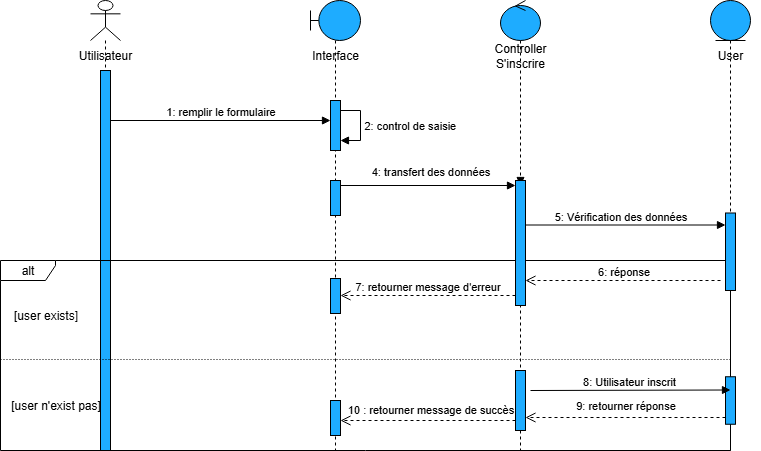
\includegraphics[width=1\linewidth]{img/signupseq.png}
    \caption{Diagramme de séquence s'inscrire}
    \label{fig:enter-label}
\end{figure}




\paragraph{Cas d’utilisation "S’Authentifier"}
\begin{itemize} [label=\textbullet]
    \item \textbf{Description textuelle du cas d’utilisation S’authentifier}
\end{itemize}
    Ce tableau 3.3 représente la description textuelle du cas d'utilisation "S'authentifier"
\begin{longtable}{|>{\raggedright\arraybackslash}p{4cm}|>{\raggedright\arraybackslash}p{11cm}|}
\hline
\textbf{Cas d’utilisation} & S’Authentifier \\
\hline
\textbf{Acteur(s)} & Administrateur \\
\hline
\textbf{Pré-condition} & L’acteur doit avoir un identifiant et un mot de passe corrects et son compte doit être vérifié. \\
\hline
\textbf{Post-condition} & Acteur authentifié \\
\hline
\textbf{Scénario nominal} &
1. L’acteur saisit son identifiant et son mot de passe. \newline
2. L’acteur clique sur le bouton de connexion. \newline
3. Le système vérifie l’existence des données. \newline
4. Le système affiche l’interface d’accueil du compte de l’acteur. \\
\hline
\textbf{Scénario alternatif} &
- Erreur de connexion au serveur. \newline
- Erreur de saisie. \newline
- Compte non vérifier ou bien compte disabled \\
\hline

\captionsetup{justification=centering}
\caption{Description textuelle du cas d’utilisation s’authentifier}
\label{tab:Description textuelle du cas d’utilisation s’authentifier}
\end{longtable}

\begin{itemize} [label=\textbullet]
    \item \textbf{Diagramme de séquence du cas d’utilisation S’authentifier}
\end{itemize}

Cette figure 3.4 elle représente le diagramme de séquence du cas d'utilisation "S'authentifier"

\begin{figure}[H]
    \centering
    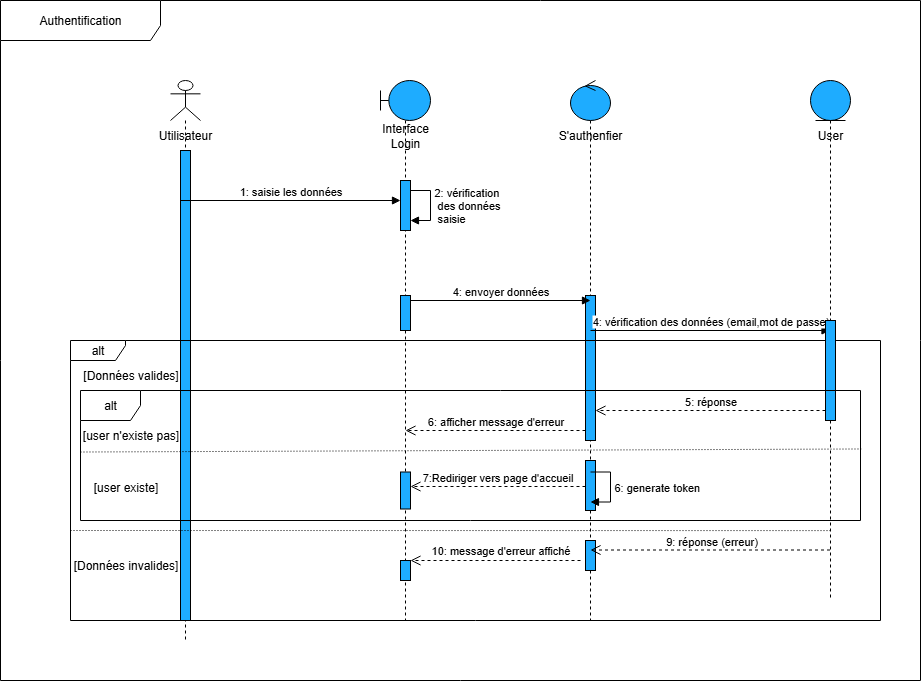
\includegraphics[width=1\linewidth]{img/loginseqdiag FinalV.png}
    \caption{Diagramme de séquence s'authentifier}
    \label{fig:enter-label}
\end{figure}


\paragraph{Cas d’utilisation "Ajouter une organisation"}
\begin{itemize} [label=\textbullet]
    \item \textbf{Description textuelle du cas d’utilisation Ajouter une organisation}
\end{itemize}
Ce tableau 3.4 représente la description textuelle du cas d'utilisation "Ajouter une organisation"

\begin{longtable}{|>{\raggedright\arraybackslash}p{4cm}|>{\raggedright\arraybackslash}p{11cm}|}
\hline
\textbf{Cas d’utilisation} & Ajouter une organisation \\
\hline
\textbf{Acteur(s)} & Administrateur \\
\hline
\textbf{Pré-condition} & Les champs du formulaire doivent être
correctement renseignés et ne doivent pas être vides. \\
\hline
\textbf{Post-condition} & Organisation Ajouté \\
\hline
\textbf{Scénario nominal} &
1. La page de création d'une organisations avec le formulaire s’affiche. \newline
2. L’acteur doit saisir les informations de l'organisation. \newline
3. Le système vérifie les données et les champs vides .\\
\hline
\textbf{Scénario alternatif} &
- Erreur de connexion au serveur. \newline
- Un message d’erreur apparaît pour lui signaler l’erreur et lui demander de corriger les données erronées . \\
\hline

\captionsetup{justification=centering}
\caption{Description textuelle du cas ajouter organisation}
\label{tab:Description textuelle du cas d’utilisation s’authentifier}
\end{longtable}

\subsection{Réalisation du Sprint 1}
Dans cette section, nous allons présenter les interfaces réalisées pour ce Sprint :

\begin{itemize} [label=\textbullet]
    \item \textbf{Interface Login :} 
    
    La figure 3.5 démontre l'interface de page login :

    \begin{figure}[H]
        \centering
        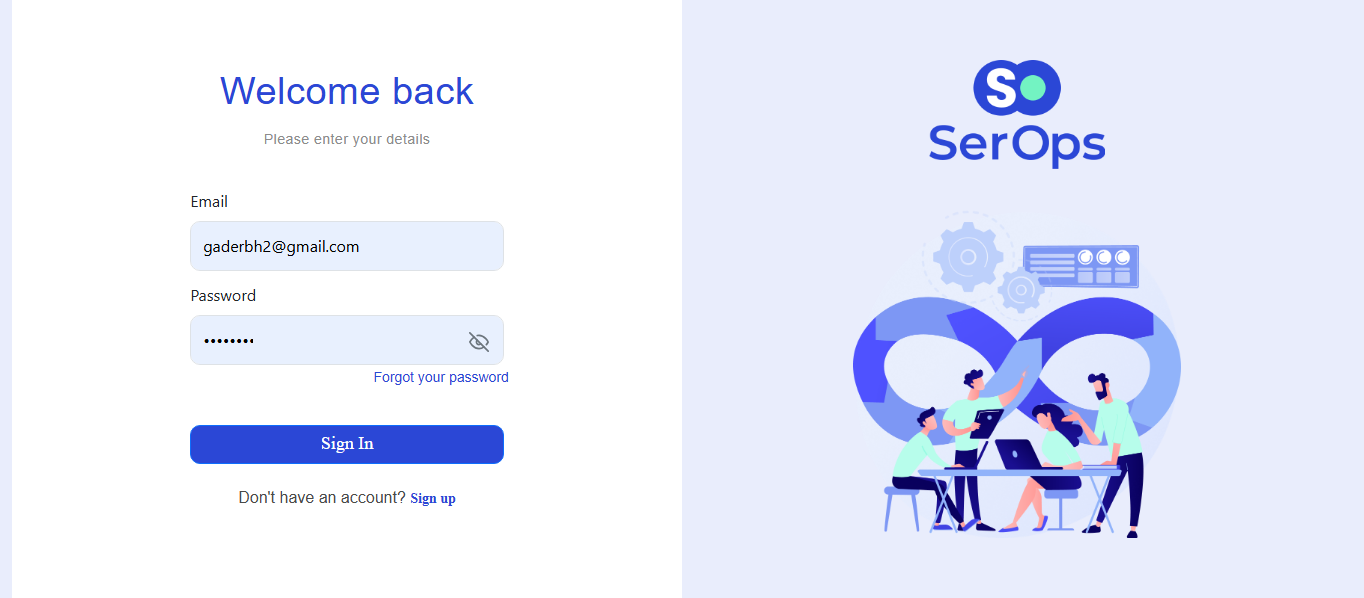
\includegraphics[width=1\linewidth]{img/InterfaceLogin.png}
        \caption{Interface login}
        \label{fig:enter-label}
    \end{figure}

    \item \textbf{Interfaces Inscription :}  
    
    La figure 3.6 représente la première étape d'inscription :

    \begin{figure}[H]
        \centering
        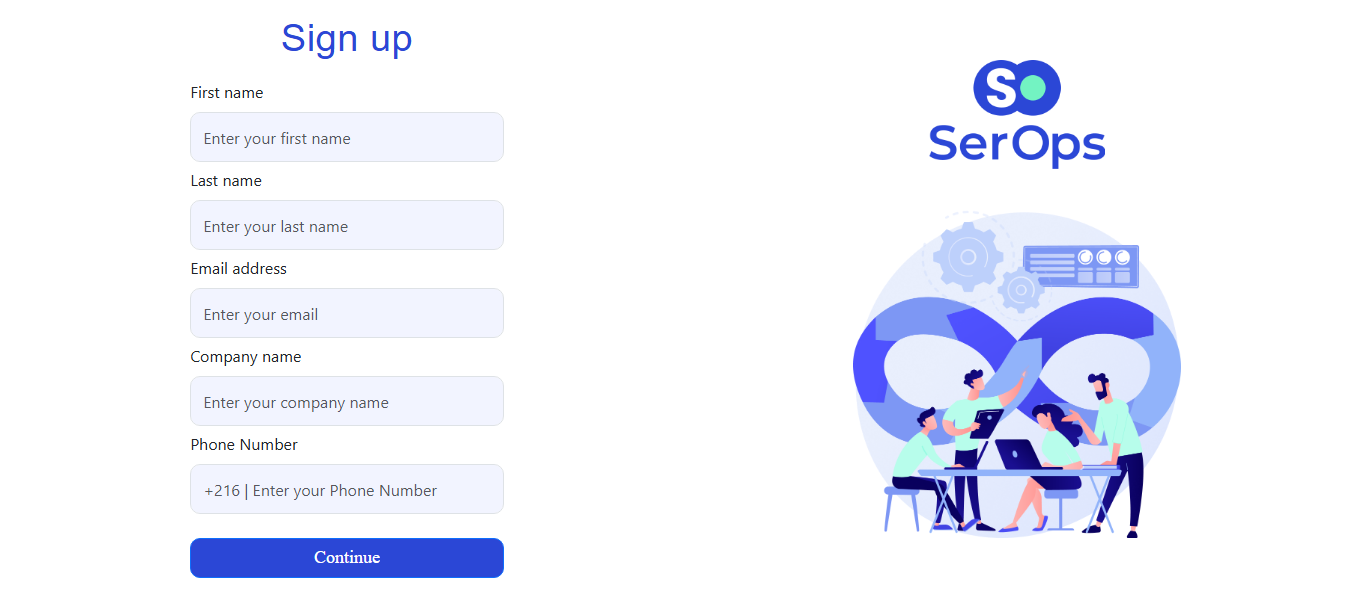
\includegraphics[width=1\linewidth]{img/SingUp1.png}
        \caption{Interface Signup 1}
        \label{fig:enter-label}
    \end{figure}
    
La figure 3.7 représente la deuxième étape d'inscription :
    
    \begin{figure}[H]
        \centering
        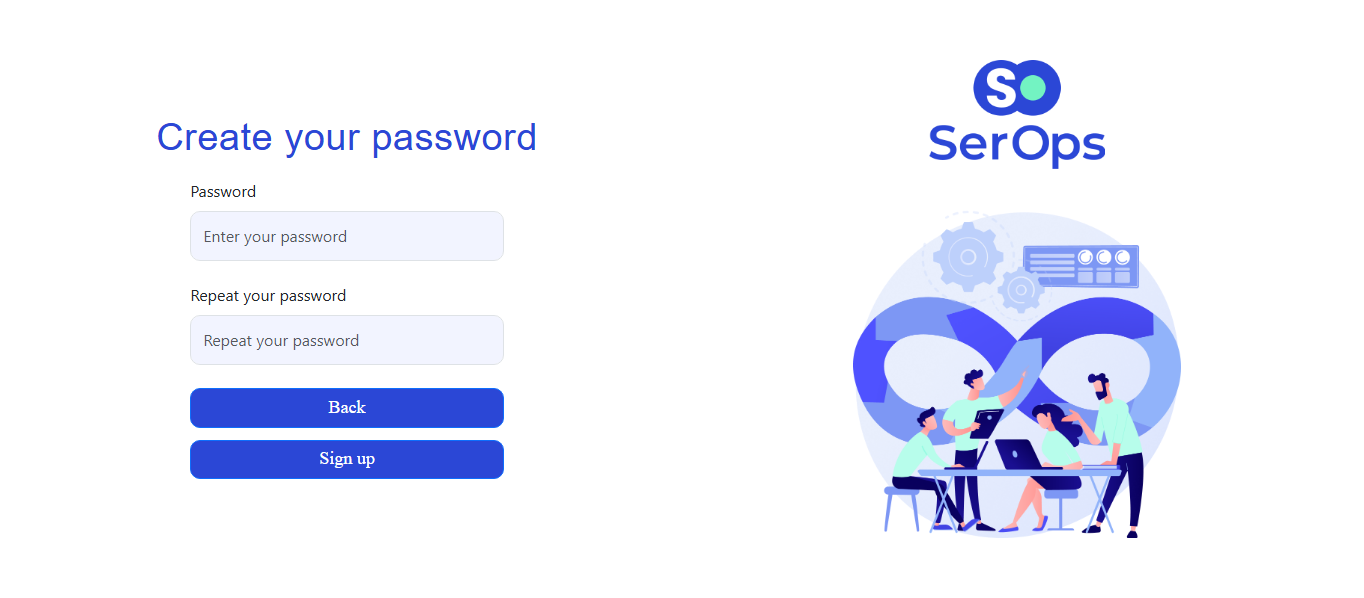
\includegraphics[width=1\linewidth]{img/SingUp2.png}
        \caption{Interface Signup 2}
        \label{fig:enter-label}
    \end{figure}
    


\item \textbf {Interface gestion organisations :}

La figure 3.8 présente l'interface dans laquelle nous permet de ajouter, modifier ou supprimer les organisations

\begin{figure}[H]
    \centering
    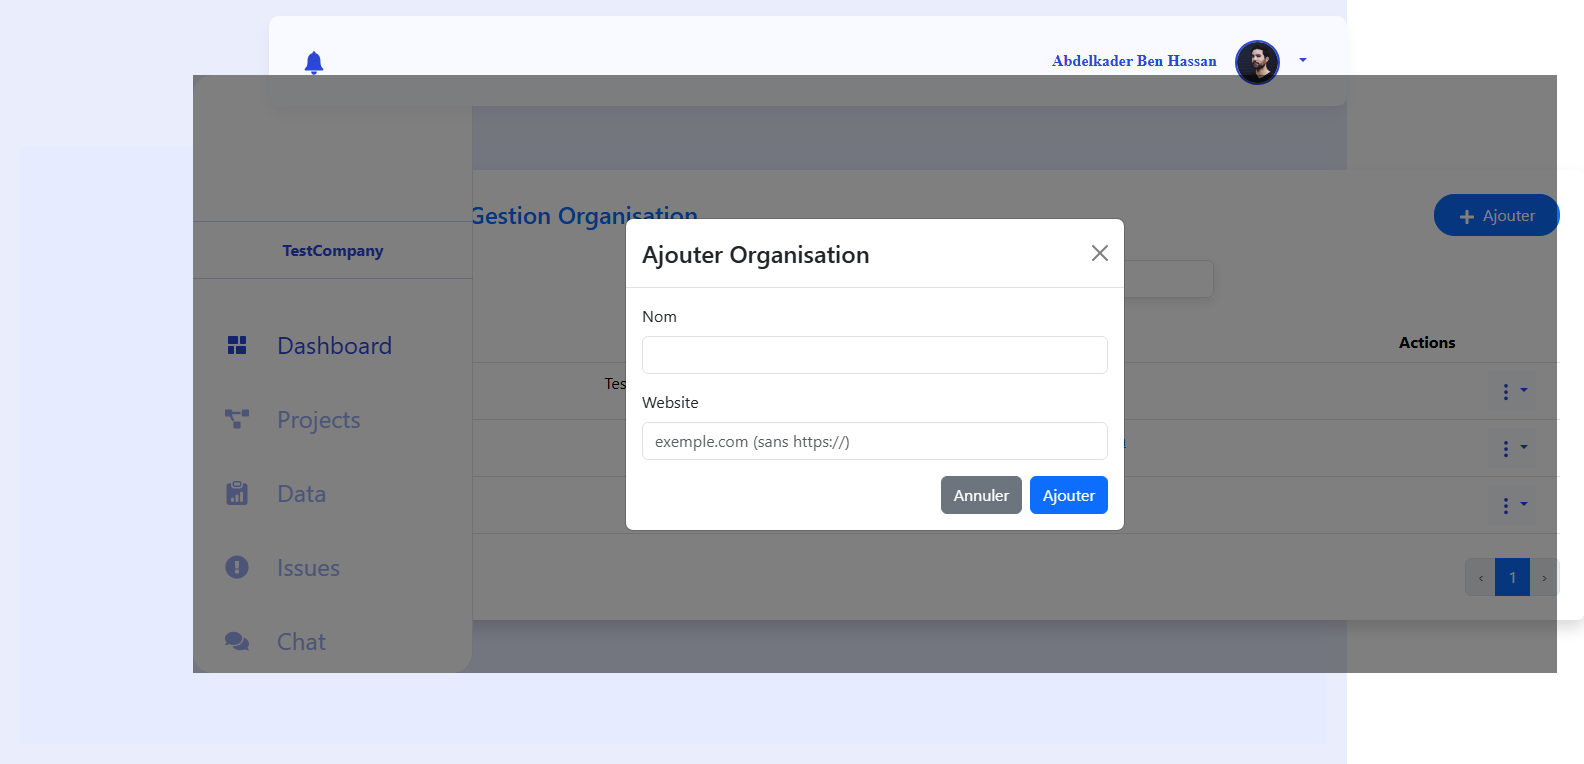
\includegraphics[width=1\linewidth]{img/Gestion Organisations.png}
    \caption{Interface Gestion Organisations}
    \label{fig:enter-label}
\end{figure}

\item \textbf{Interface Modifier profil : }

La figure 3.9 présente l'interface dans laquelle nous permet de modifier les informations :

\begin{figure}[H]
    \centering
    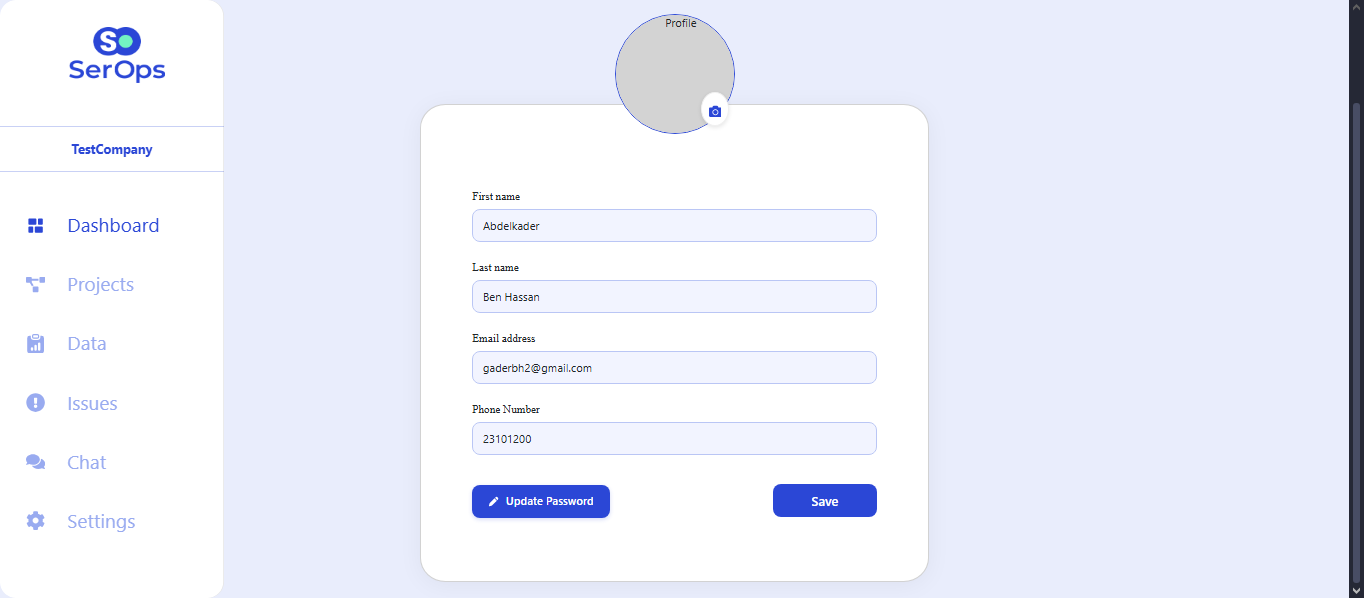
\includegraphics[width=1\linewidth]{img/profile.png}
    \caption{Interface modifier profil}
    \label{fig:enter-label}
\end{figure}

\end{itemize}

\section{Sprint 2} 
\subsection{Objectifs du sprint 2}
Ce sprint a pour objectif de mettre en place les fonctionnalités essentielles de gestion des médicaments et des traitements. Il permettra aux utilisateurs de créer et gérer leur inventaire personnel de médicaments, soit en scannant les codes-barres pour récupération automatique des informations, soit par saisie manuelle. Le sprint introduit également la gestion complète des traitements médicaux avec leurs prescriptions associées, permettant aux utilisateurs de créer, modifier et suivre leurs traitements. De plus, la boîte à pharmacie virtuelle sera mise en place pour gérer l'inventaire des médicaments disponibles, suivre les dates d'expiration et l'historique des achats. Ce sprint vise ainsi à fournir une base solide pour le suivi médical personnel et familial.
\subsection{Backlog Sprint 2}

\begin{table}[H]
\centering
\renewcommand{\arraystretch}{1.4}
\resizebox{\textwidth}{!}{%
\begin{tabular}{|
>{\centering\arraybackslash}m{1cm}|
>{\centering\arraybackslash}m{4cm}|
>{\centering\arraybackslash}m{1cm}|
m{6cm}|
>{\centering\arraybackslash}m{2cm}|
>{\centering\arraybackslash}m{2cm}|
>{\centering\arraybackslash}m{2cm}|}
\hline
\textbf{ID} & \textbf{Module} & \textbf{ID} & \textbf{User Story} & \textbf{Priorité} & \textbf{Complexité} & \textbf{Nb jours} \\
\hline

\multirow{3}{*}{2} & \multirow{3}{4cm}{Gestion des médicaments}
& 2.1 & En tant qu'utilisateur, je veux consulter les détails de mes médicaments & Haute & 3 & 1 \\
\cline{3-7}
& & 2.2 & En tant qu'utilisateur, je veux ajouter un médicament en scannant son code QR ou code à barre pour obtenir automatiquement ses informations & Haute & 5 & 3 \\
\cline{3-7}
& & 2.3 & En tant qu'utilisateur, je veux ajouter un médicament en saisissant ses informations manuellement & Haute & 3 & 2 \\
\hline

\multirow{3}{*}{4} & \multirow{3}{4cm}{Gestion des traitements}
& 4.1 & En tant qu'utilisateur, je veux ajouter un traitement avec au moins une prescription & Haute & 5 & 2 \\
\cline{3-7}
& & 4.2 & En tant qu'utilisateur, je veux modifier un traitement & Haute & 5 & 2 \\
\cline{3-7}
& & 4.8 & En tant que responsable du groupe, je veux consulter les traitements d'un utilisateur & Haute & 5 & 1 \\
\hline

\multirow{2}{*}{5} & \multirow{2}{4cm}{Gestion des prescriptions}
& 5.1 & En tant qu'utilisateur, je veux ajouter une ou plusieurs prescriptions pour un traitement & Haute & 5 & 2 \\
\cline{3-7}
& & 5.6 & En tant que responsable, je veux ajouter une prescription à un utilisateur & Haute & 5 & 2 \\
\hline

\multirow{2}{*}{7} & \multirow{2}{4cm}{Gestion des boîtes}
& 7.1 & En tant qu'utilisateur, je veux ajouter un médicament à ma boîte & Haute & 5 & 2 \\
\cline{3-7}
& & 7.4 & En tant qu'utilisateur, je veux consulter les médicaments présents dans ma boîte & Moyenne & 3 & 1 \\
\hline

\end{tabular}%
}
\captionsetup{justification=centering}
\caption{Backlog Sprint 2}
\label{tab:BacklogSprint2}
\end{table}

Le tableau 3.5 représente le backlog du Sprint 2.

\subsection{Etude conceptuelle du sprint 2}
\subsubsection{Use Case sprint 2}
La figure 3.10 représente le diagramme de cas d'utilisation du sprint 2


\begin{figure}[H]
    \centering
    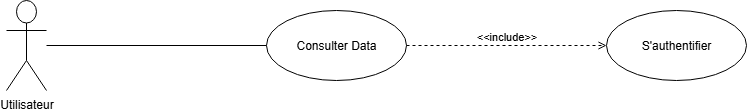
\includegraphics[width=1\linewidth]{img/Sprint2UseCaseFV.png}
    \caption{use case du Sprint 2}
    \label{fig:enter-label}
\end{figure}

\subsubsection{Diagramme de classes Sprint 2}


La figure 3.11 représente le diagramme de classes du deuxième sprint

\begin{figure}[H]
    \centering
    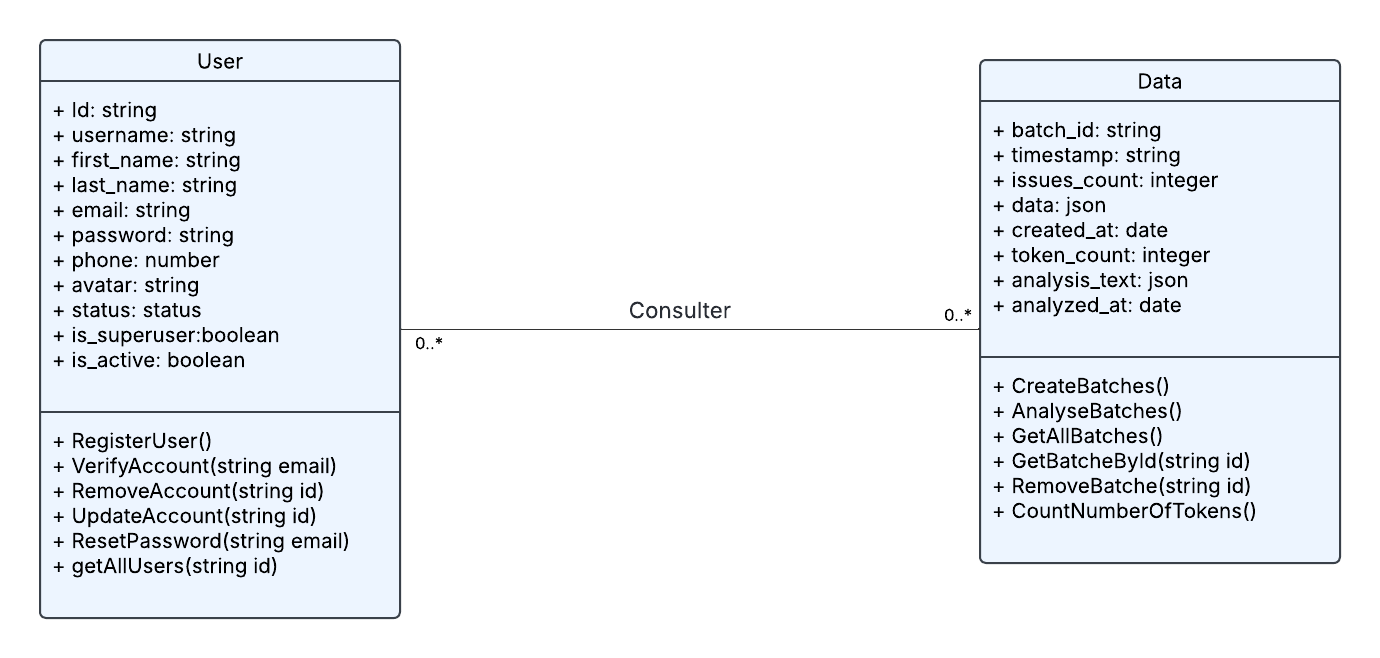
\includegraphics[width=1.15\linewidth]{img/sprint 2 classes.png}
    \caption{Diagramme de classes Sprint 2}
    \label{fig:enter-label}
\end{figure}

\subsubsection{Descriptions textulle  des cas d’utilisation du sprint 2}
\paragraph{Cas d'utilisation consulter data}
\begin{itemize} [label=\textbullet]
    \item \textbf{Description textuelle du cas d’utilisation consulter Data}
\end{itemize} 
Le tableau 3.6 représente la description textuelle du cas d'utilisation "s'inscrire"

\begin{longtable}{|>{\raggedright\arraybackslash}p{4cm}|>{\raggedright\arraybackslash}p{11cm}|}
\hline
\textbf{Cas d’utilisation} & Consulter Data \\
\hline
\textbf{Acteur(s)} & Utilisateur \\
\hline
\textbf{Pré-condition} & L'utilisateur doit être authentifié et ses données doivent exister. \\
\hline
\textbf{Post-condition} & Data Affiché \\
\hline
\textbf{Scénario nominal} &
1. L'utilisateur visite la page qui affiche les data. \newline
2. L’utilisateur choisi un batche a consulter . \newline
3. Le système affiche les logs liée a se batche avec les filtres de severité des log et de type de data (metriques ou bien logs).\\
\hline
\textbf{Scénario alternatif} &
- Erreur de connexion au serveur. \newline
- Pas de data disponible . \\
\hline

\captionsetup{justification=centering}
\caption{Description textuelle du cas d’utilisation s’inscrire}
\label{tab:Description textuelle du cas d’utilisation s’authentifier}
\end{longtable}


\begin{itemize} [label=\textbullet]
    \item \textbf{Diagramme de sequences consulter les data}
\end{itemize}
La figure 3.12 représente la diagramme de séquence "liste Data"

\begin{figure}[H]
    \centering
    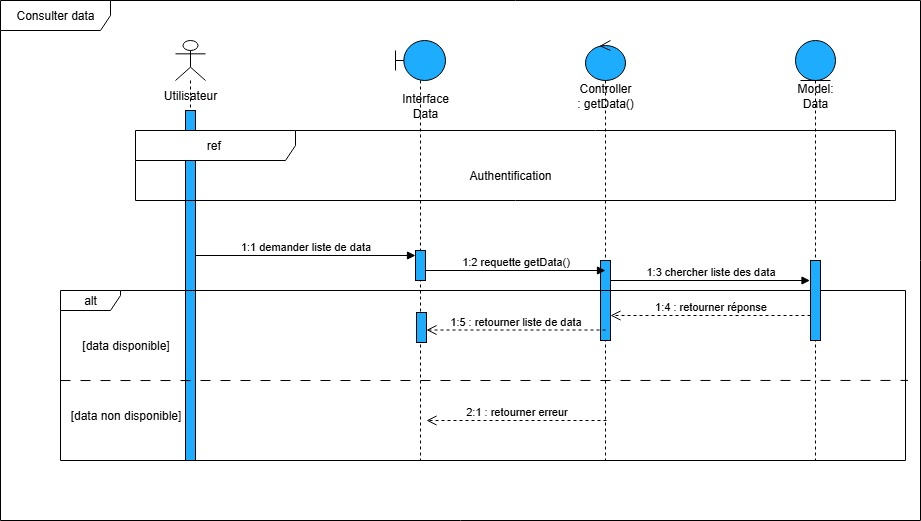
\includegraphics[width=1\linewidth]{img/batcheslistfinalversion.jpg}
    \caption{Diagramme de séquence liste data}
    \label{fig:enter-label}
\end{figure}


\subsection{Réalisation du Sprint 2} 
Dans cette section, nous allons présenter les interfaces réalisées pour cette sprint


\begin{itemize} [label=\textbullet]
    \item \textbf{Interfaces pour consulter les Data}


Ces interfaces constituent des outils essentiels qui nous permettent non seulement de consulter en temps réel les logs et les métriques, mais aussi d’analyser en profondeur le comportement du système, de détecter les anomalies, et d’optimiser les performances globales de l’infrastructure.


\clearpage

La figure 3.13 représnte l'interface des batches dans laquelle on peut trouver la liste des batches créer

\begin{figure}[H]
    \centering
    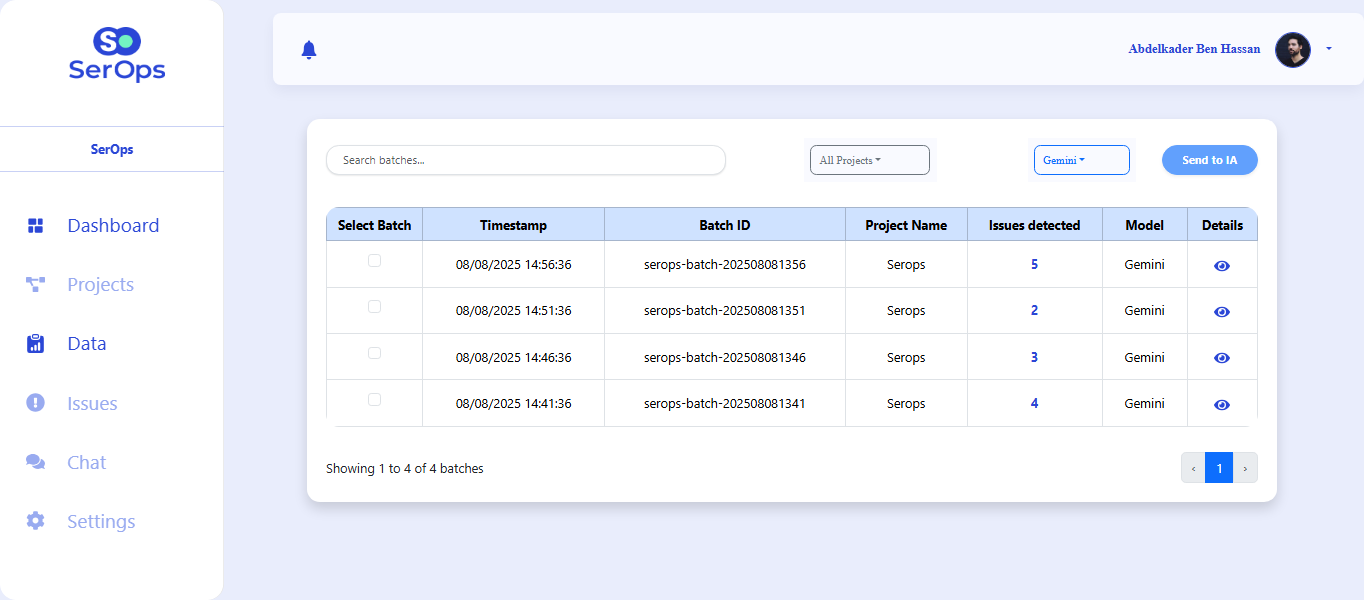
\includegraphics[width=1\linewidth]{img/DataPage.png}
    \caption{Interface Data}
    \label{fig:enter-label}
\end{figure}

La figure 3.14 représnte l'interfaces des logs d'un batche dans laquelle on peut consulter les détails des logs d'un batch

\begin{figure}[H]
    \centering
    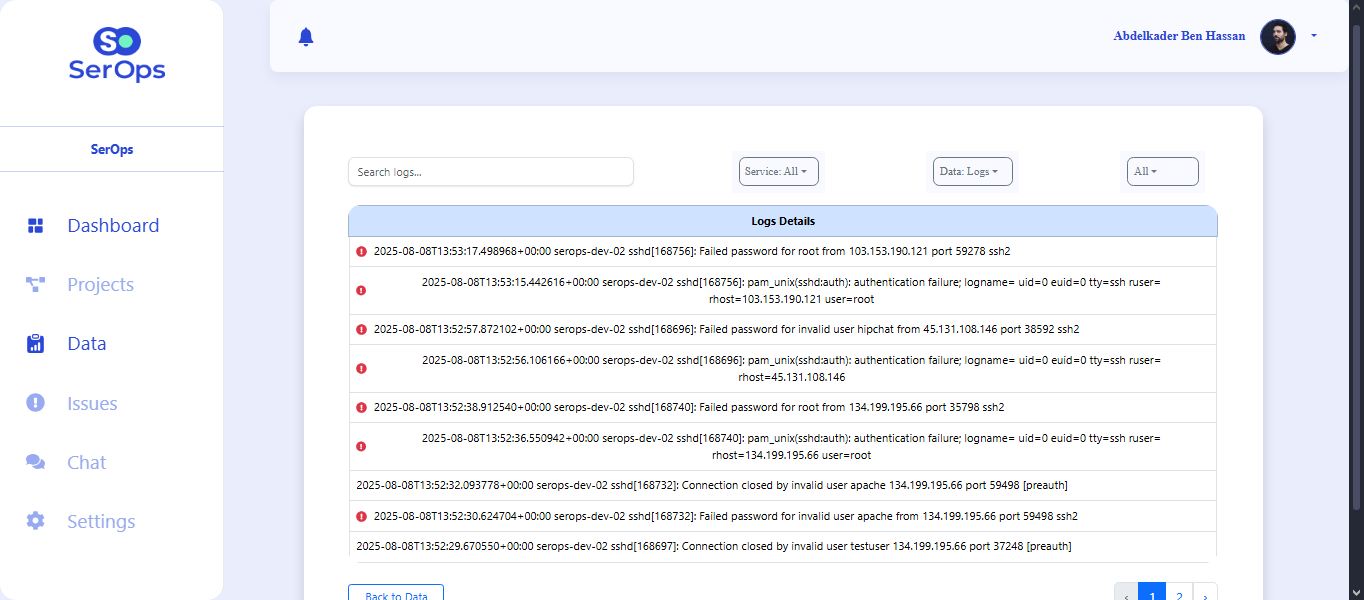
\includegraphics[width=1\linewidth]{img/LogsPage.png}
    \caption{Interface Logs}
    \label{fig:enter-label}
\end{figure}

\clearpage

La figure 3.15 représente l'interface d'utilisation mémoire d'un serveur 

\begin{figure}[H]
    \centering
    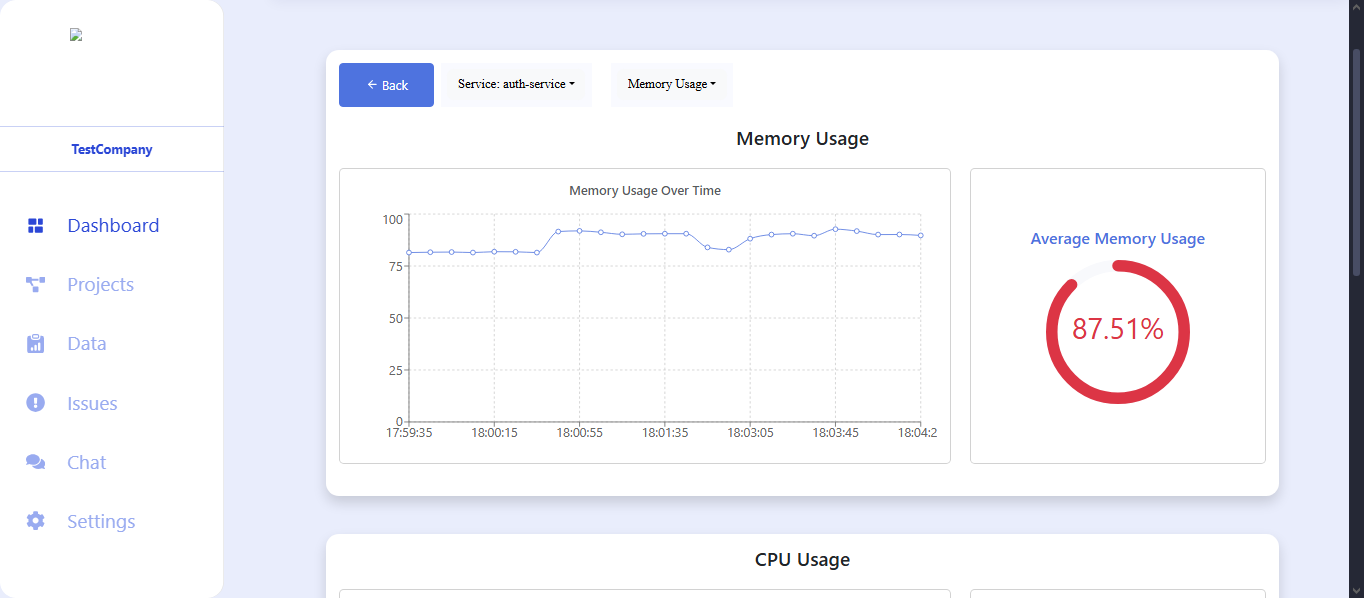
\includegraphics[width=1\linewidth]{img/MetMemory.png}
    \caption{Interface Memory metriques}
    \label{fig:enter-label}
\end{figure}

La figure 3.16 représente l'interface d'utilisation processeur d'un serveur 

\begin{figure}[H]
    \centering
    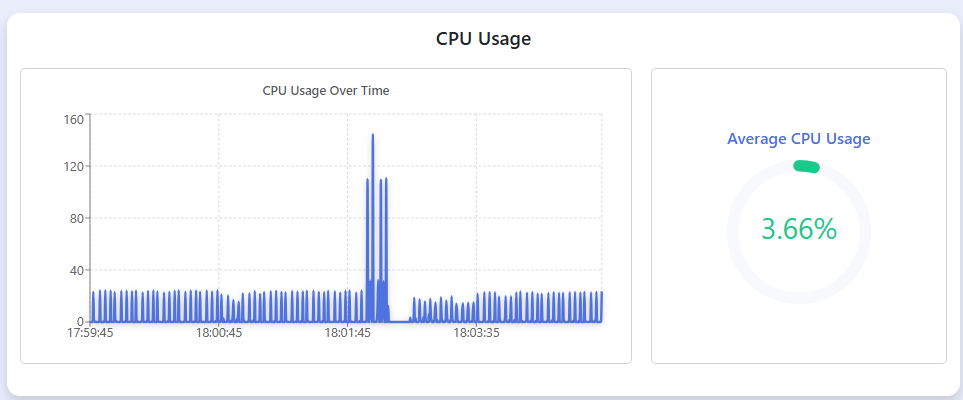
\includegraphics[width=1\linewidth]{img/MetCpu.png}
    \caption{Interface cpu métriques}
    \label{fig:enter-label}
\end{figure}

\end{itemize}

\section{Conclusion} 
Nous avons présenté un aperçu détaillé de la release 1 de notre projet, qui regroupe les travaux réalisés lors des sprints 1 et 2. Cette version intègre la conception et le développement de l’application d’authentification, ainsi que les fonctionnalités de gestion du profil , des logs, des métriques et des organisations.
Dans le chapitre suivant, nous analyserons en détail le déroulement du release 2.